\documentclass{article}
\usepackage[utf8]{inputenc}
\usepackage[spanish]{babel}
\usepackage{amsmath}
\usepackage{amssymb}
\usepackage{mathtools}

\title{Control Sistemas Mecatronicos}
\author{BMJIvan }

\begin{document}

\maketitle

%UNIDAD I
\section{Conceptos fundamentales}

\[
    \text{Aplicaciones}
    \left\{
        \begin{array}{l}
            \text{Transporte de fluidos} \\
            \text{Conversión de la energía} \\
            \text{Acondicionamiento de ambiente} \\
            \text{Turbomáquinaria} \\
            \text{Transporte (vehicular)} 
        \end{array}
    \right.
\]

\[
    \begin{array}{c}
         \text{Áreas de}  \\
         \text{mecánica de fluidos}
    \end{array}
    \left\{ 
        \begin{array}{l}
             \text{Aerodinámica} \\
             \text{Hidráulica} \\ 
             \text{Hidrología} \\
             \text{Metrología}
        \end{array}
    \right.    
    \begin{array}{l}
        \\
        \left\{
            \begin{array}{l}
                \text{Hidráulica de potencia} \\
                \text{Redes de tubería} \\
                \text{Neumática}
            \end{array}
        \right. \\
        \\
        \\
    \end{array}
\]

\[
    \begin{array}{c}
         \text{Técnicas o}  \\
         \text{métodos o analíticos}
    \end{array}
    \left\{ 
        \begin{array}{l}
             \text{Analíticos} \\
             \text{Experimentales} \\ 
             \text{Computacionales} 
        \end{array}
    \right.    
    \begin{array}{l}
        \left\{
            \begin{array}{l}
                \text{Diferenciales} \\
                \text{Diferenciales} 
            \end{array}
        \right.\\
        \\
        \\
    \end{array}
\]

Presión, esfuerzo normal: Genera deformaciones lineales
\[
    P = \lim \frac{ \Delta F_{n} }{ \Delta A } = \frac{ dF_{n} }{ dA }
\]

Esfuerzo cortante: Genera deformaciones angulares 
\[
    \tau = \lim \frac{ \Delta F_{t} }{ \Delta A } = \frac{ dF_{t} }{ dA }
\]

\subsection{Propiedades de los fluidos}
Densidad 
\[ 
    \rho = \frac{ m }{ v } \;\; \Big[ {}^{ kg }/_{ m^3 }. {}^{ lbm }/_{ pie^3 }, {}^{ slug }/_{ pie^3 } \Big]
\]

Peso especifico
\[
    \gamma = \frac{ W_{g} }{ v } = \frac{ mg }{ v } = \rho g \;\; \Big[ {}^{ N }/_{ m^3 }, {}^{ lb }/_{ pie^3 } \Big]
\]

Densidad relativa 
\[
    sg = GE = \rho_{r} = \frac{ \rho_{fluido} }{ \rho_{H_{2}O \;\; T = 4^{o}C} }
\]

Viscosidad dinámica o absoluta
\[
    \mu = \frac{ \tau }{{}^{ d \Vec{u} }/{ dy }} \;\; \frac{ \text{Esfuerzo cortante} }{ \text{Gradiente de velocidad} }
\]
\[
    \mu = \frac{ \tau y }{ \Vec{u} } \;\; \Big[ {}^{N \cdot s }/{ m^{2}, {}^{ lb \cdot s }/{ pie^2 } } \Big]
\]

Viscosidad cinemática
\[
    \nu = \frac{ \mu }{ \rho } \;\; \Big[ {}^{ m^{2} }/{ s }, {}^{ pie^{2} }/{ s } \Big]
\]

\subsection{Gases ideales}

Proceso adiabático: Aquel proceso en el que no se gana ni pierde calor, es decir, cuenta con un aislamiento térmico. 

En proceso adiabático reversible no hay transferencia de calor y por lo tanto el proceso es isoentrópico.

Un proceso adiabático irreversible no es isoentropico. 
\[
    \begin{split}
        \forall & : \text{ Volumen} \\
        \nu & : \text{ volumen especifico \( \frac{ \forall }{ m } = \frac{ 1 }{ \rho } \)}
    \end{split}
\]

\begin{enumerate}
    \item Ley de Boyle y Mariotte
        \[
            \begin{split}
                \text{Si }T & = constante \\
                P \; & \alpha \; \frac{ 1 }{ \forall } \\
                P \forall & = C \\
                P_{ 1 } \forall_{ 1 } & = P_{ 2 } \forall_{ 2 }  
            \end{split}
        \]
    \item Ley de Charles
        \[
            \begin{split}
                \text{Si }P & = constante \\
                \forall\; & \alpha \; T \\
                \frac{ \forall }{ T } & = C \\
                \frac{ \forall_{1} }{ T_{1} } & = \frac{ \forall_{2} }{ T_{2} } 
            \end{split}
        \]
    \item Ley de Gay - Lussac
        \[
            \begin{split}
                \text{Si } \forall & = constante \\
                P \; & \alpha \; T \\
                \frac{ P }{ T } & = C \\
                \frac{ P_{1} }{ T_{1} } & = \frac{ P_{2} }{ T_{2} } 
            \end{split}
        \]
    \item 
        \[
            \begin{split}
                \frac{ P \forall }{ T } & = C \\
                \frac{ P_{1} \forall_{1} }{ T_{1} } & = \frac{ P_{2} \forall_{2} }{ T_{2} } \\
                \frac{ P \nu }{ T } & = nR_{u} \\
                R_{u} & = \frac{ P \forall }{ Tn }
            \end{split}
        \]
        Donde 
        \[
            \begin{split}
                P & = 1 \text{ atmósfera} \\
                T & = 0^{o}C = 273.15K \\
                n & = 1 \text{ kmol} \\
                \forall & = 22.413 m^{3} \\
                R_{u} & = 8.314 {}^{kJ}/_{kmol \cdot K} \\
                n & = \frac{ m }{ M } \; \frac{ \text{ masa } }{ \text{ masa molar } } \\
                R & = \frac{ R_{u} }{ M } \text{ constante del gas }
            \end{split}
        \]
        Entonces 
        \[
            \begin{split}
                R_{u} & = \frac{ P \forall }{ T {}^{m}/{M} } = \frac{ MP \forall }{ Tm } \\
                m \frac{ R_{u} }{ M } & = \frac{ P \forall }{ T } \\
                \frac{ P \forall }{ T } & = mR \\
                P \forall & = TmR \\
                P \frac{ \forall }{ m } & = TR \\
                P \nu & = TR \\
                P & = \frac{ 1 }{ \nu } TR = \rho TR \\
                \frac{ P }{ \rho } & = TR
            \end{split}
        \]
\end{enumerate}

\subsection{ Velocidad sonica o acústica y viscosidad }

A partir de 1
\[
    dp \; \alpha \; - \frac{ d \forall }{ \forall } \\
    dp = -E_{v} \frac{ d \forall }{ \forall }
\]

Donde \( E_{v} \) es el modulo de compresibilidad o modulo volumétrico. \\ 
De la definición de masa
\[
    \begin{split}
        m & = \rho \forall \\
        dm & = \rho dv + d\rho \forall, \;\; dm = 0 \\
        -\rho d\forall & = d\rho \forall \\
        - \frac{ d \forall }{ \forall } & = \frac{ d\rho }{ \rho }
    \end{split}
\]

por lo tanto
\[
    dp = E_{v} \frac{ d\rho }{ \rho }
\]

\[
    C = \sqrt{ \frac{ dp }{ d\rho } } = \sqrt{ \frac{ E_{v} }{ \rho } } \;\; \text{Velocidad del sonido a través de líquidos}
\]
\[
    \begin{split}
        K & = \frac{ C_{p} }{ C_{\nu} } = 1.4 \\
        R & = C_{p} - C_{ \nu } \;\; \Big[ {}^{kJ}/{ kg \cdot K } \Big] \\
        R & = .287 {}^{kJ}/{ kg \cdot K } \\
        C & = \sqrt{ \frac{ k_{p} }{ \rho } } = \sqrt{KTR} \\
        E_{v} & = P \; \text{ Proceso isotérmico} \\
        E_{v} & = KP \; \text{ Proceso isoentropico} \\
    \end{split}
\]
Líquidos incompresibles \( \rho = constante \) \\
Líquidos compresibles \( \rho \not = constante \) 
\[
    \begin{split}
        \text{Mach } & = \frac{ \Vec{v} }{ C } \; \frac{ \text{velocidad fluido} }{ \text{ velocidad de sonido } } \\
        \text{Mach } & \leq .3 \; \text{flujo de gas incompresible} \\
        \text{Mach } & \geq .3 \; \text{flujo compresible}
    \end{split}
\]

\[
    \overbrace{ \frac{ \mu }{ \rho } }^{ \text{Dinámica} } = \overbrace{ v }^{ \text{Cinemática} }
\]

\[
    \begin{split}
        \mu & = \text{ constante o \( 0 \) ideal o no viscoso} \\
        \mu & \not = \text{ constante o \( 0 \) real o viscoso }
    \end{split}
\]

\[
    \begin{array}{c}
         \text{Fluido de acuerdo}  \\
         \text{al comportamiento} \\
         \text{de la \( \mu \)}
    \end{array}
    \left\{ 
        \begin{array}{l}
             \text{Newtoniano} 
                \left\{
                    \begin{array}{l}
                        \tau \; \alpha \; \frac{ d\theta \text{ deformación} }{ dt } \to 
                            \begin{array}{l}
                                \text{ley de viscosidad} \\
                                \text{de Newton}
                            \end{array}
                    \end{array}
                 \frac{ d\theta }{ dt } = \frac{ d\Vec{v} }{ dy } 
                 \right.\\ 
             \text{No Newtoniano} 
                \left\{
                    \begin{array}{l}
                         \tau \text{ no } \; \alpha \; \frac{ d\theta }{ dt } \to \text{ Series de potencias }
                    \end{array}
                \right.\\ 
             \text{Visco-elástico} 
                \left\{
                    \begin{array}{l}
                         \text{Comportamiento Newtoniano}  \\
                         \text{y no Newtoniano}
                    \end{array}
                \right.
        \end{array}
    \right.    
\]

Número de Raynolds
\[
    NR_{E} = \frac{ \text{Fuerzas de inercia} }{ \text{Fuerzas viscosas} } = \overbrace{ \frac{ \rho \Vec{v} D }{ \mu } }^{ \text{Dinámica} } = \overbrace{ \frac{ \Vec{v}D }{ \forall } }^{ \text{Cinemática} }
\]

\[
    \begin{array}{c}
         \text{Flujo viscoso}
    \end{array}
    \left\{ 
        \begin{array}{l}
             \text{flujo laminar} 
                \left\{
                    \begin{array}{l}
                        NR_{E} \leq 2000 \;\; (2300) 
                    \end{array}
                 \right.\\ 
             \text{flujo transición} 
                \left\{
                    \begin{array}{l}
                         2000 \leq NR_{E} \leq 4000
                            \begin{array}{l}
                                \text{puede ser}\\
                                \text{laminar o turbulento}
                            \end{array}
                    \end{array}
                \right.\\ 
             \text{flujo turbulento} 
                \left\{
                    \begin{array}{l}
                         NR_{E} \geq 4000
                    \end{array}
                \right.
        \end{array}
    \right.    
\]

\[
    P_{abs} = P_{atm} \pm P_{rel} \to P_{ \text{manométrica}}
\]

\[
    \begin{split}
        Mach & > 1 \; \text{ supersónico} \\
        Mach & > 5 \; \text{ hipersónico} \\
        Mach & < 1 \; \text{ sursónico} \\
        Mach & = 1 \; \text{ sónico} \\
        Mach & \leq 1 \; \text{ transónico}
    \end{split}
\]

\[
    \dot{ \forall } = \frac{ \forall }{ t } = \Vec{ v } A \to \; \text{ caudal}
\]

\[
    \begin{split}
        \rho_{ gasolina } = 680 {\;}^{ kg }/_{ m^{3} } \;\; & E_{v} = 1.3 \times 10^{9} {\;}^{ N }/_{ m^{2} } \\
        \rho_{ Hg } = 13600 {\;}^{ kg }/_{ m^{3} } \;\;& E_{v} = 2.85 \times 10^{10} {\;}^{ N }/_{ m^{2} } \\
        \rho_{H_{2}O \; mar} = 1030 {\;}^{ kg }/_{ m^{3} } \;\;& E_{v} = 2.34 \times 10^{9} {\;}^{ N }/_{ m^{2} } \\
    \end{split}
\]

\subsection{Esfuerzo cortante}
\[
    \begin{split}
        \tau \; & \alpha \; \frac{ du }{ dt } = \frac{ \Vec{v} }{ dy } \\
        \tau & = \mu \frac{ d\Vec{ v } }{ dy } \\
        \tau \int_{ 0 }^{ h }dy & = \mu \int_{ 0 }^{ \Vec{v} } \\
        \tau h & = \mu \Vec{ v } \\
        \tau & = \mu \frac{ \Vec{ v } }{ h } \\
        \tau & = \lim_{\Delta A \to 0} \frac{ \Delta F_{t} }{ \Delta A } = \frac{ dF_{t} }{ dA } \\
        \tau & = \frac{ F_{t} }{ A }
    \end{split}
\]
Donde \( F_{v} \) es la fuerza viscosa o tangente
\[
    \begin{split}
        \mu \frac{ \Vec{v} }{ h } = \frac{ F_{v} }{ A }\\
        F_{v} = \frac{ \mu \Vec{v} A }{ h }    
    \end{split}
\]

caso 1: 
\[
    \begin{split}
        A & = \pi d L \\
        h & = \frac{ D - d }{ 2 } \\
        F_{v} & = \frac{ 2 \pi d L \Vec{v} \mu }{ D - d }
    \end{split}
\]

caso 2:
\[
    \begin{split}
        F_{v} & = W \sin{ \theta } \\
        h & = \frac{ \mu \Vec{v} A }{ W \sin{ \theta } }
    \end{split}
\]

*tablas líquidos y gases: mecánica de fluidos Pottev

\subsection{Tensión o esfuerzo superficial} 
\[
    \sigma_{s} = \frac{ F_{ \text{tensión} } }{ l } \;\; \Big[ {}^{ W }/_{ m }, {}^{ lb }/_{ pie } \Big]
\]
\[ 
    \begin{split}
        \sum F_{y} & = 0 \\
        F_{rsy} - Wg & = 0 \\
        \sigma_{s} \pi D \cos{ \theta } - \rho \forall g & = 0 \\
        \sigma_{s} \pi D \cos{ \theta } - \rho g \frac{ \pi D^{2} }{ 4 } h & = 0 \\
        \sigma_{s} \cos{ \theta } & = \frac{ \rho g D h }{ 4 } \\
        h & = \frac{ 4 \sigma_{s} \cos{ \theta } }{ \rho g D }
    \end{split}
\]

\section{Grupos de procesos y áreas de conocimientos}

\subsection{Grupos de procesos de la dirección de proyectos}

\begin{enumerate}
    \item Inicialización: Autorización para comenzar dicho proyecto.
    
    \item Planeación: Establecer el alcance, refinar objetivos. 
    
    \item Ejecución: Procesos para completar el trabajo.
    
    \item Monitoreo y control: Regular desempeño del proyecto.
    
    \item Cierre: Todas las actividades para completar el trabajo.
\end{enumerate}

\begin{figure}[h!]
    \centering
        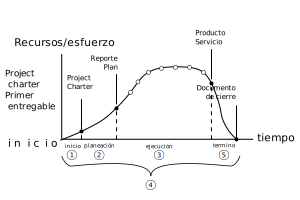
\includegraphics[scale=0.30]{Manufactura Integrada por Computadora Figuras/Figura02 Ciclo de Vida de Proyecto.png}
        \caption{Ciclo de vida de proyecto}
\end{figure}

\subsection{Áreas  de conocimiento}

\begin{enumerate}
    \item Gestión de la integración del proyecto: Tomar decisiones en cuanto a la asignación de recursos. Balancear objetivos y manejar las interdependencias entre áreas. 
    
    \item Gestión del alcance del proyecto: Definir y controlar lo que se incluye y lo que no.
    
    \item Gestión del tiempo del proyecto: Definir y secuenciar actividades, estimar recursos y duración de las actividades. 
    
    \item Gestión de los costos del proyecto: estimar, presupuestar y controlar los costos. 
    
    \item Gestión de la calidad del proyecto: Procesos y actividades para se satisfaga las necesidades. 
    
    \item Gestión de los recursos humanos del proyecto: Procesos que organizan, gestionan y conducen el proyecto. 
    
    \item Gestión de las comunicaciones del proyecto: Procesos que organizan, gestionan y conducen el proyecto.
    
    \item Gestión de riesgos del proyecto: Procesos para identificar, analizar, planear respuestas a los riesgos. 
    
    \item Gestión de las adquisiciones del proyecto: Procesos de compra de productos o servicios. administración de contratos y ordenes. 
    
    \item Gestión de los interesados del proyecto: Proceso para identificar personas, grupos que pueden afectar o ser afectados por el proyecto. 
\end{enumerate}

Linea base de un proyecto: Punto de medida de tiempo, alcance y recursos. 

\begin{figure}[h!]
    \centering
        \includegraphics[scale=0.30]{Manufactura Integrada por Computadora Figuras/Figura03 Triangulo de Hierro.png}
        \caption{Triangulo de hierro}
\end{figure}

\subsection{Controlabilidad y observabilidad de sistemas lineales}

Sea el sistema 
\[(1)
    \left\{
        \begin{array}{lll}
            \dot{x}(t) = \overbrace{ A }^{ \text{estabilidad} }x(t) + \underbrace{ B }_{ \textbf{controlabilidad} }u(t) \\
            y(t) = Cx(t)
        \end{array}
    \right.
\]

donde 
\[
    \begin{split}
        X & : n \times 1 \\
        A & : n \times n \\
        B & : n \times m \;\; entradas \\
        u & : m \times 1 \\
        C & : p \times n \\
        y & : P \times 1 \;\; salidas
    \end{split}
\]

Controlabilidad: existencia de una entrada \( u(t) \) tal que cada variable de estado se pueda manipular de manera independiente, es decir, las entradas cambian las variables.

Observabilidad: Consiste en determinar el estado inicial a partir de la salida \( y(t) \), es decir, las condiciones iniciales afectan la salida.

\begin{figure}[h!]
    \centering
    \begin{subfigure}[b]{0.45\linewidth}
        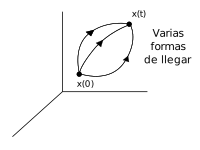
\includegraphics[scale=0.25]{Control de Sistemas Mecatronicos Figuras/01 Controlabilidad}
        \caption{Controlabilidad}
    \end{subfigure}
    \begin{subfigure}[b]{0.45\linewidth}
        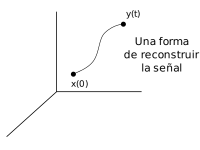
\includegraphics[scale=0.25]{Control de Sistemas Mecatronicos Figuras/02 Observabilidad}
        \caption{Observabilidad}
    \end{subfigure}
\end{figure}

Definición 1. El sistema (1) es controlable si existe \(u(t)\) tal que para todo estado inicial \( x_{0}=x(0) \) y todo estado final \(x_{f}=x(T)\), el sistema puede llevarse de \( x_{0} \) a \( x_{f} \) en tiempo finito.

\section{Ecuaciones básicas de los fluidos en forma integral}

\subsection{Transformación de un sistema a volumen de control}

%figura

\begin{itemize}
    \item Volumen de control y el sistema ocupan las regiones 1 y 2 en el tiempo \( t \)
    \item Sistema en el instante \( t \) ocupa los volúmenes 1 y 2
    \item Sistema en el instante \( t + \Delta t \) ocupa los volúmenes 2 y 3
\end{itemize}

\[
    N_{sist} = \underbrace{ \int_{m} \eta dm }_{
        \begin{array}{cc}
            \text{masa} \\
            \text{(sistema)}
        \end{array} } 
    = \underbrace{ \int_{\forall} \eta \rho d \forall }_{
        \begin{array}{cc}
            \text{volumen} \\
            \text{(sistema)}
        \end{array} }
\]

Donde
\[
    \begin{split}
        N: \; & \; \text{Propiedad extensiva del sistema} \\ 
        \eta: & \; \text{Propiedad intensiva del sistema}
    \end{split}
\]

\[
    \begin{split}
        \frac{ dN }{ dt } \Big|_{ \text{sist} } & = \lim_{ \Delta t \to 0 } \frac{ N_{sist}(t + \Delta t) - N_{sist}(t) }{ \Delta t } \\
        & = \lim_{ \Delta t \to 0 } \frac{ N_{2}(t + \Delta t) + N_{3}(t + \Delta t) - N_{2}(t) - N_{1}(t) + N_{1}(t + \Delta t) - N_{1}(t + \Delta t) }{ \Delta t } \\
        & = \lim_{ \Delta t \to 0 } \frac{ (N_{2} + N_{1})(t + \Delta t) - (N_{2} + N_{1}) }{ \Delta } + \lim_{ \Delta t \to 0 } \frac{ N_{3}(t + \Delta t) - N_{1}(t + \Delta t) }{ \Delta t } \\
        & = \lim_{ \Delta t \to 0 } \frac{ N_{ \forall_{c} }(t + \Delta t) - N_{ \forall_{c}(t) }}{ \Delta } + \lim_{ \Delta t \to 0} \frac{ N_{3}(t + \Delta t) - N_{1}(t + \Delta t) }{ \Delta t } \\
        & = \frac{ dN_{ \forall_{c} } }{ dt } + \lim_{ \Delta t \to 0 } \frac{ N_{3}(t + \Delta t) - N_{1}(t + \Delta t) }{ \Delta t }
    \end{split}
\]

%figura

\[
    \begin{split}
        d \forall_{1} & = - \hat{n} dA \cdot \Vec{v}_{1} \cdot \Delta t \\
        d \forall_{3} & = \hat{n} dA \cdot \Vec{v}_{3} \cdot \Delta t \\
        N_{3}(t + \Delta t) & = \int_{A_{3}} \eta \hat{n} \rho \Vec{v} \Delta t dA \\
        N_{1}(t + \Delta t) & = - \int_{A_{1}} \eta \hat{n} \rho \Vec{v} \Delta t dA
    \end{split}
\]

\subsection{Teorema del transporte de Reynolds}
Lagrange \( \to \) Euler

\[
    \begin{split}
        \frac{ dN }{ dt } \Big|_{ \text{sist} } & = \frac{ d }{ dt } \int_{\forall_{c}} \eta \rho d\forall + \int_{A_{3}} \eta \rho \Vec{v}_{3} dA_{3} - \int_{A_{1}} \eta \rho \Vec{v}_{1} dA_{1} \\
        & = \frac{ \partial }{ \partial t } \int_{ \forall_{c} } \eta \rho d\forall + \int_{sc} \eta \rho \Vec{v}dA \\
        & = \underbrace{ \frac{ \partial }{ \partial t } \int \int \int \eta \rho \Vec{v} dA}_{
            \begin{scriptsize}
                    \begin{array}{cc}
                        \text{Como cambia dentro} \\
                        \text{del volumen de} \\
                        \text{control}
                    \end{array}
            \end{scriptsize}
        } + 
        \underbrace{ \frac{ \partial }{ \partial t } \int \int \eta \rho \Vec{v} dA}_{
            \begin{scriptsize}
                    \begin{array}{cc}
                        \text{Flujo de propiedad extensiva neta} \\
                        \text{a través de la superficie de control} \\
                        \text{control}
                    \end{array}
            \end{scriptsize}
        }
    \end{split}
\]

\subsection{Propiedades extensivas e intensivas}

\begin{table}[h!]
    \centering
    \begin{tabular}{|c|c|} \hline
        \text{Extensiva (N)} & \text{Intensiva ( \( \eta) \)} \\ \hline
        \text{m: masa} & \text{1: ecuación de continuidad} \\ \hline
        \text{E: energía} & e: energía especifica \\ \hline
        \text{\( \Vec{P} \): cantidad de momento lineal} & \text{\( \Vec{v} \): velocidad} \\ \hline
        \text{\( \Vec{H} \): cantidad de momento angular} & \text{\( \Vec{v} \times \Vec{r} \): velocidad angular } \\ \hline
        \text{S: entropía total} & \text{s: entropía especifica} \\ \hline
    \end{tabular}
\end{table}

\subsection{Masa}
\[
    \frac{ dm }{ dt } \Big|_{ \text{sist} } = \frac{ \partial }{ \partial t } \int_{ \forall_{c} } \rho d\forall + \underbrace{ \int_{ sc_{ent} }^{ sc_{sal} } }_{ 
    \begin{scriptsize}
            \begin{array}{cc}
                \text{flujo de} \\
                 \text{masa neto}
            \end{array}
    \end{scriptsize}
    } \rho \Vec{v} dA
\]

\[
    \frac{ dm }{ dt } \Big|_{ \text{sist} } = 0
\]

\[
    \frac{ d }{ dt } \int_{\forall_{c}} \rho d\forall = \int_{ sc_{ent} }(\rho \Vec{v} dA)_{ent} - \int_{ sc_{sal} }(\rho \Vec{v} dA)_{sal} 
\]

\subsection{Energía}
Función de trayectoria no son condición de estado
\[
    \begin{split}
        \dot{Q}_{neto} & = \dot{Q}_{ent} - \dot{Q}_{sal} \\
        \dot{W}_{neto} & = \dot{W}_{sal} - \dot{W}_{sal}
    \end{split}
\]

\[
    \begin{split}
        \frac{ dE }{ dt }\Big|_{sist} & = \dot{Q} - \dot{W} \\
        \frac{ dE }{ dt }\Big|_{sist} & = \dot{Q}_{neto} + \dot{W}_{neto}
    \end{split}
\]

\[
    \begin{split}
        \frac{ dE }{ dt }\Big|_{sist} & = \frac{ d }{ dt } \int_{ \forall_{c} } e\rho d\forall + \int_{sc} e \rho \Vec{v} dA \\
        \dot{Q}_{neto} + \dot{W}_{neto} & = \frac{ d }{ dt } \underbrace{ \int_{\forall_{c}} e \rho d\forall }_{
            \begin{scriptsize}
                    \begin{array}{cc}
                        \text{Cambio de} \\
                         \text{energía total}
                    \end{array}
            \end{scriptsize} } + 
        \underbrace{ \int_{sc} e \rho \Vec{v} dA }_{
            \begin{scriptsize}
                    \begin{array}{cc}
                        \text{Flujo de} \\
                         \text{energía}
                    \end{array}
            \end{scriptsize} }
    \end{split}
\]

\[
    \frac{ d }{ dt } \int_{ \forall_{c} } \rho d \forall = \int_{sc_{ent}} \rho \Vec{v} dA - \int_{sc_{sal}} \rho \Vec{v} dA
\]

\[
    \dot{Q}_{neto} + \dot{W}_{neto} = \frac{ d }{ dt } \int_{ \forall_{c} } e \rho d\forall + \int_{sc_{salida}} (e \rho \Vec{v} dA)_{sal} - \int_{sc_{entrada}} (e \rho \Vec{v} dA)_{ent}
\]

\[
    \begin{split}
        e_{s \; cerrado} & = u + \frac{ 1 }{ 2 } v^{2} + gz \\
        e_{s \; abierto} & = P_{v} + u + \frac{ 1 }{ 2 } \Vec{v} + gz
    \end{split}
\]

\subsection{Momento lineal}
\[
    \begin{split}
        \frac{ dN }{ dt }\Big|_{sist} & = \frac{ d }{ dt } \int_{ \forall_{c} } \eta \rho d\forall + \int_{sc} \eta \rho \Vec{v} dA, \;\; N = \Vec{P} \;\; \eta = \Vec{v} \\
        \frac{ d\Vec{P} }{ dt }\Big|_{sist} & = \frac{ d }{ dt } \int_{ \forall_{c} } \Vec{v} \rho d\forall + \int_{sc} \Vec{v} \rho \Vec{v} dA \\
        \underbrace{ \sum F_{s} }_{ \text{superficie} } + \underbrace{ \sum F_{B} }_{ \text{cuerpo} } & = \frac{ d }{ dt } \int_{ \forall_{c} } \Vec{v} \cdot \rho d\forall + \int_{sc} \Vec{v} \cdot \rho \Vec{v} dA \\
        \sum F_{sx} + \sum F_{Bx} & = \frac{ d }{ dt } \int_{\forall_{c}} \Vec{u}_{x} \cdot \rho d\forall + \int_{sc} \Vec{u}_{x} \cdot \rho \Vec{v} dA \\
        \sum F_{sy} + \sum F_{By} & = \frac{ d }{ dt } \int_{\forall_{c}} \Vec{u}_{y} \cdot \rho d\forall + \int_{sc} \Vec{u}_{y} \cdot \rho \Vec{v} dA \\
    \end{split}
\]

\subsection{Momento angular}

\[
    \begin{split}
        N & = \Vec{ H } \to  \eta = \Vec{ r } \times \Vec{ v } \\
        \frac{ d\Vec{ H } }{ dt } \Big|_{sist} & = \frac{ d }{ dt } \int_{ \forall } (\Vec{r} \times \Vec{v} ) \cdot \rho d\forall + \int_{sc} (\Vec{r} \times \Vec{v} ) \cdot \rho \Vec{v} dA \\
        \sum M_{s} + \sum M_{g} & = \frac{ d }{ dt } \int_{ \forall } (\Vec{r} \times \Vec{v} ) \cdot \rho d\forall + \int_{sc} (\Vec{r} \times \Vec{v} ) \cdot \rho \Vec{v} dA \\
        S_{sistema} + S_{generada} & = \frac{ d }{ dt } \int_{ \forall } S \cdot \rho d\forall + \int_{sc} S \cdot \rho \Vec{v} dA
    \end{split}
\]

\subsection{Para ejercicios}

\[
    \begin{split}
        dh = 0 \;\; \text{permanente o estacionario} \\
        \frac{ dh }{ dt } > 0 \;\; y \;\; \frac{ dh }{ dt } < 0 \;\; \text{transitorio}
    \end{split}
\]

Flujo permanente: turbina, compresores, ventiladores
\[
    \int_{ \forall } e \rho d\forall = 0
\]

Proceso adiabático: no hay transferencia de calor
\[
    w_{ent} = 0
\]

Se le debe proporcionar potencia a una bomba

\subsection{Eficiencias}

Generador eléctrico

\[
    \begin{split}
        \eta_{ \text{eólica} } & = \frac{ P_{mec} }{ \Delta\dot{E}_{c} } \;\; \Delta \dot{E}_{c}: \; \text{ cambio de energía cinética} \\
        \eta_{ \text{generador eléctrico} } & = \frac{ \dot{W}_{elec} }{ P_{mec} } \\
        \eta_{mec} = \eta_{ \text{eólica} } \eta_{ \text{generador eléctrico} }
    \end{split}
\]

Bomba
\[
    \begin{split}
        \Delta u & = 0 \\
        \dot{Q}_{sal} & = 0 \\
        \dot{Q}_{ent} & = 0 \\
        \dot{W}_{sal} & = 0 \\
    \end{split}
\]

\[
    \begin{split}
        \eta_{B} & = \frac{ \Delta \dot{E}_{p} }{ P_{mec} } = \frac{ P_{ \text{hidráulica} } }{ P_{mec} } \\
        \eta_{elec} & = \frac{ P_{mec} }{ \dot{W}_{elec} } = \frac{ P_{mec} }{ P_{elec} } \\
        \eta_{mec} & = \eta_{B} \cdot \eta_{elct}
    \end{split}
\]

Motor
\[
    \begin{split}
        \eta_{ \text{motor combustión interna} } & = \frac{ P_{mec} }{ \dot{Q}_{combustible} } \\
        & = \frac{ \tau W }{ \dot{Q} } = \frac{ \tau W }{ \dot{m}_{c} \cdot PCI } \\
        & = \frac{ \tau W }{ \rho \dot{ \forall } \cdot PCI } \\
        PCI: & \text{ poder calorífico especifico}  
    \end{split}
\]

Boiler: calentador de agua
\[
    \begin{split}
        \eta_{Boiler} & = \frac{ \dot{Q}_{H_{2}O} }{ \dot{Q}_{combus} } = \frac{ \dot{m}_{H_{2}O} (T_{2} - T_{1} ) }{ \dot{m}_{combus} \cdot PCI } \\
        \dot{Q}_{combus} : & \;\; \text{energía térmica} \\
        \dot{m}_{combus} : & \;\; \text{cuando no hay cambio de fase}
    \end{split}
\]

Calentador de agua eléctrico 
\[
    \begin{split}
        \eta_{CA} = \frac{ \dot{Q}_{H_{2}O} }{ \dot{W}_{elec} } = \frac{ \dot{m}_{ H_{2}O } }{ E \cdot I \cdot f.p } \\
        (T_{2} - T_{1}): & \;\; por temperaturas
    \end{split}
\]

Generador de vapor
\[
        \eta_{G.V} = \frac{ \dot{Q}_{vapor} }{ \dot{Q}_{comb} } = \frac{ \dot{m}_{vapor} (h_{2} - h_{1}) }{ \dot{m}_{comb} \cdot PCI }
\]

otras eficiencias

\begin{itemize}
    \item refrigerador 
    \item colector solar
    \item turbina: vapor, gas, hidráulica
    \item compresor 
    \item ventilador
    \item reactor nuclear 
    \item panel fotovoltaico
    \item horno
\end{itemize}

\section{Arquitectura funcional}

\subsection{consideraciones para generar la arquitectura funcional}
\begin{enumerate}
    \item Las funciones deben ser claras.
    \item Entender la conexión y comunicación entre funciones. 
\end{enumerate}

\subsection{Esta compuesta por los siguientes tres modelos}
\begin{enumerate}
    \item Jerarquía de funciones (FBS: Function, Behaviour, Structure)
    \item Relación entre funciones (IDEF-0: Integration Definition for Function Modeling)
    \item Comportamiento ente funciones (EFFBD: Enhanced Function Flow Block Diagram)
\end{enumerate}

Considerando los atributos de sistemas mecatrónicos, y las funciones generales del sistema propuesto. Las funciones genéricas del sistema mecatrónico son:
\begin{itemize}
    \item F10: Medición de parámetros del sistema y entorno.
    \item F20: Detección de errores del sistema.
    \item F30: Interacción con el usuario.
    \item F40: Administración de decisiones, proceso de aprendizaje, manejo del conocimiento.
    \item F50: Acondicionamiento de entradas y salidas.
    \item F60: Almacenamiento de información.
    \item F70: Comunicación interna y externa.
    \item F80: Recuperación de la funcionalidad.
    \item F90: Desempeñar funciones propias del sistema.
    \item F100: Soporte y protección.
    \item F110: Administración energética (alimentación, conversión, distribución, almacenamiento)
\end{itemize}

\subsection{Principales errores al generar la arquitectura funcional}
\begin{itemize}
    \item Mejorar dominios, incluir funciones que describen el comportamiento, sistemas o componentes físicos en la misma arquitectura. Por ejemplo: HMI (Human Machine Interface), cuando la función que desempeña es la interacción con el usuario.
    \item Inconsistencias en la salida de las funciones, deben representar la transformación.
    \item Elegir nombres confusos e incorrectos para las funciones, entradas o salidas.
    \item Que la función represente o desarrolle más de una función.
    \item La arquitectura (modos de operación) no representa el comportamiento completo del sistema.
    \item Las salidas del sistema y las funciones no representan las expectativas y necesidades del sistema.
\end{itemize}

\subsection{Modelo EFFBD}
Permite en la arquitectura funcional determinas el comportamiento que tiene un sistema a través del flujo de funciones. Este flujo está definido como el trayecto que siguen las entradas y salidas a lo largo de transformaciones.

\subsubsection{Generalidades}
Las funciones se representan con bloques, estos tienen un indicador (el mismo que se obtiene de la estructura funcional).

Existen dos tipos de entradas y salidas, las entradas "pasivas" y las entradas "activas".

Las activas se refieren a que mantienen su flujo activo mientras se realiza la transformación. Las pasivas ya no transmiten flujo hasta que termine la transformación. 

\subsection{Forma Canonica Controlable}
Ejercicio: demostrar que la propiedad de controlabilidad es invariante para cualquier transformación de similtud

Se considera la transformación de similitud
\[
    (1) X=P^{-1}z
\]

donde \( P \) es invertible
Se toma el sistema 
\[
    (2)
    \left\{
        \begin{array}{lll}
            \dot{x}(t) = Ax(t) + Bu(t)\\
            y(t) = Cx(t)
        \end{array}
    \right.
\]

Se sustituye (1) en (2) para conseguir \( P^{-1}\dot{z} = AP^{-1}z+Bu \), y asi, obtener el sistema
\[
    (3)
    \left\{
        \begin{array}{lll}
            \dot{z}(t) =
                \overbrace{PAP^{-1}}^{\tilde{A}}+ 
                \overbrace{PBu}^{\tilde{B}}\\
            y(t) = CP^{-1}
        \end{array}
    \right.
\]

donde \( A \) y \( PAP^{-1} \) son invariantes, se tiene que \( \lambda (A) = \lambda(PAP^{-1}) \) debido a que \( P \) es invertible, entonces \(rango(\tilde{C}) = rango(C)\).

Se obtiene la matriz de controlabilidad para los sitemas (2) y (3) respectivamente.

\[
    (4)\;\;
    C=[B , AB , A^{2}B , \ldots , A^{n-1}B]
\]
\[
    (5)\;\;
    \tilde{C}=[\tilde{B} , \tilde{A}\tilde{B} , \tilde{A}^{2}\tilde{B} , \ldots , \tilde{A}^{n-1}\tilde{B}]
\]

Considerando que \( (PAP^{-1})^{n} = PA^{n}P^{-1} \), se sustituye las matrices similares de (3) en (5)
\[
    \begin{split}
        \tilde{C} & = [PB, PAP^{-1}PB, PA^{2}P^{-1}PB, \ldots, PA^{n-1}P^{-1}PB] \\
        \tilde{C} & = P[B, AB, A^{2}B, \ldots, A^{n-1}B] \\
        \tilde{C} & = PC 
    \end{split}
\]

Lo que se busca es la matriz \( P \), por lo tanto, de la ecuación anterior se puede despejar de la siguiente forma
\[
    \begin{split}
        \tilde{C} & = PC \\
        \tilde{C}\tilde{C}^{-1} & = PC\tilde{C}^{-1} \\
        I & = PC\tilde{C}^{-1} \\
        P^{-1}I & = C\tilde{C}^{-1} \\
        P^{-1} & = C\tilde{C}^{-1}\;\;(6)
    \end{split}
\]

Ahora se tomará el sistema de entradas y salidas
\[
    \begin{split}
        y^{n}(t) + a_{1}y^{n-1}(t) + \ldots + a_{n}y(t) & = b_{1}u^{n-1}(t) + \ldots + b_{n}u(t) \\
        \mathcal{L} \{ y^{n}(t) + a_{1}y^{n-1}(t) + \ldots + a_{n}y(t) \} & = \mathcal{L} \{ b_{1}u^{n-1}(t) + \ldots + b_{n}u(t) \}\\
        y(s)s^{n} + a_{1}y(s)s^{n-1} + \ldots + a_{n}y(s) & = b_{1}u(s)s^{n-1} + \ldots + b_{n}u(s)\\
        y(s) (s^{n} + a_{1}s^{n-1} +\ldots + a_{n} ) & = u(s) (b_{1}s^{n-1} + \ldots + b_{n})
    \end{split}
\]

Se escribe la función de transferencia como 
\[
    g(s) = \frac{y(s)}{u(s)} = \frac{ b_{1}s^{n-1} + \ldots + b_{n} }{ s^{n} + a_{1}s^{n-1} +\ldots + a_{n} } = \frac{N(s)}{D(s)}
\]

Si consideramos una función de transferencia racional (sin retardo) y estrictamente propia (orden del denominador mayor que el numerador)
\[
    g(s)=N(s)D(s)^{-1}
\]
donde N(s) y D(s) son polinomios. Por lo tanto, la función de transferencia se puede escribir como 
\[
    g(s) = \frac{y(s)}{u(s)} = N(s)D(s)^{-1}
\]

La salida del sistema se puede escribir como 
\[
    y(s) = N(s)D(s)^{-1}u(s)
\]

donde \( v(s) = D(s)^{-1}u(s) \). Entonces la entrada y la salida se pueden escribir como 
\[
    \begin{split}
        u(s) & = D(s)v(s) \\
        y(s) & = N(s)v(s)
    \end{split}
\]

Se definen las variables de estado de la siguiente forma
\[ 
    \begin{bmatrix}
        X_{1}(s) \\
        X_{2}(s) \\
        \vdots \\
        X_{n-1}(s) \\
        X_{n}(s)
    \end{bmatrix}
    =
    \begin{bmatrix}
        S^{n-1} \\
        S^{n-2}\\
        \vdots \\
        S \\
        1
    \end{bmatrix} v(s)
\]

entonces las variables de estado se pueden escribir como

\[
    \begin{split}
        X_{n} & = v(s)\\
        X_{n-1} = sv(s) & = sX_{n}(s)\\
        X_{n-2}(s) = S^{2}v(s) =s(sv(s)) & = sX_{n-1}(s)\\
        &\;\;\vdots\\
        X_{2}(s) & = sX_{3}(s)\\
        X_{1}(s) & = sX_{2}(s)
    \end{split}
\]

Si se sustituyen las variables de estado en la entrada se obtiene lo siguiente
\[
    u(s) = sX_{1}(s) + a_{1}X_{1}(s) + \ldots + a_{n}X_{n}(s)
\]

Se despeja \( sX_{1}(s) \)
\[
    sX_{1}(s) = -a_{1}X_{1}(s) - \ldots - a_{n}X_{n} + u(s)
\]

Entonces es posible escribir el espacio de estados como
\[
    \begin{bmatrix}
        SX_{1}(s) \\
        SX_{2}(s) \\
        \vdots \\
        SX_{n}(s)
    \end{bmatrix}
    =
    \underbrace{
        \begin{bmatrix}
        -a_{1} & -a_{2} & \cdots & -a_{n}\\
        1 & 0 & \cdots & 0 \\
        \vdots & \ddots & \cdots & \vdots \\
        0 & \cdots & 1 & 0
        \end{bmatrix}
                }_{\tilde{A}}
    \begin{bmatrix}
        X_{1}(s) \\
        X_{2}(s) \\
        \vdots \\
        X_{n}(s)
    \end{bmatrix}
    +
    \underbrace{
        \begin{bmatrix}
        1\\
        0\\
        \vdots\\
        0
        \end{bmatrix}
                }_{\tilde{B}}
     u(s)
\]

Según la definición de la matriz similar de controlabilidad
\[
    \tilde{C} = [
    \tilde{B},
    \tilde{A}\tilde{B},
    \tilde{A}^{2}\tilde{B},
    \cdots,
    \tilde{A}^{n-1}\tilde{B} ]
\]

Se usará una matriz de 3*3 para encontrar un patrón
\[
    \tilde{C} = 
    \begin{bmatrix}
        1 & -a_{1} & -a_{1}^{2}-a_{2} \\
        0 & 1 & -a_{1} \\
        0 & 0 & 1
    \end{bmatrix}
\]

La inversa esta dada por
\[
    \tilde{C}^{-1} = 
    \begin{bmatrix}
        1 & a_{1} & a_{2} \\
        0 & 1 & a_{1} \\
        0 & 0 & 1
    \end{bmatrix}
\]

Por lo tanto, la inversa de la matriz similar de controlabilidad se puede expresar como 
\[
    \tilde{C}^{-1} = 
    \begin{bmatrix}
        1 & a_{1} & a_{2} & \cdots & a_{n-1} \\
        0 & 1 & a_{1} & \cdots & a_{n-2}\\
        \vdots & \ddots & \ddots & \ddots & \vdots\\
        0 & 0 & 0 & \ddots & a_{1}\\
        0 & 0 & 0 & \cdots & 1
    \end{bmatrix}
\]

Considerando la matriz de controlabilidad 
\[
    C = [B, AB, A^{2}B, \cdots, A^{n-1}B ]
\]

La ecuación (6) se puede escribir como
\[
    P^{-1} =
    [B, AB, A^{2}B, \cdots, A^{n-1}B ]
    \begin{bmatrix}
        1 & a_{1} & a_{2} & \cdots & a_{n-1} \\
        0 & 1 & a_{1} & \cdots & a_{n-2}\\
        \vdots & \ddots & \ddots & \ddots & \vdots\\
        0 & 0 & 0 & \ddots & a_{1}\\
        0 & 0 & 0 & \cdots & 1
    \end{bmatrix}
\]

\section{Dominio físico}
El dominio físico es la transformación de las funciones que el sistema debe desempeñar en componentes físicos. Estos pueden ser partes, ensambles, módulos, dispositivos, sistemas.

La representación del dominio físico es mediante un diagrama a bloques, denominado arquitectura funcional, con base en las funciones generadas de un sistema mecatrónico, se propone la siguiente arquitectura. 

\begin{figure}[h!]
    \centering
        \includegraphics[scale=0.22]{Proyecto Integrador Figuras/22 Dominio fisico.png}
        \caption{Dominio físico}
\end{figure}

Con base en teoría de sistemas, un sistema mecatrónico se puede considerar como un "sistema de sistemas" (SoS), y a su vez el sistema que tiene mayor impacto en el sistema mecatrónico se denomina como "sistema de interés" (SoI).

\begin{figure}[h!]
    \centering
        \includegraphics[scale=0.20]{Proyecto Integrador Figuras/23 Dominio Logico y Fisico.png}
        \caption{Dominio lógico y físico}
\end{figure}

%UNIDAD II
\section{UNIDAD II}
\subsection{Diseño de sistemas de control en espacios de estado}

De manera general un sistema de control se define

donde \( u:\) señal de control, \(y:\) señal disponible. Se asume que la referencia y la salida son conocidas.

En funcion de \( r \) se definen los siguientes problemas de control:

\begin{enumerate}
    \item Regulación: se considera que \( r \) es constante
    \item Seguimiento de trayectoria: En este caso \( y \) es una función variante con el tiempo
    \item Seguimiento de modelo de referencia
\end{enumerate}

Los sistemas de control se clasifican en dos tipos principales
\begin{enumerate}
    \item En lazo abierto\\\\
    La señal de control es independiente de la salida.
    \item En lazo cerrado o retroalimentado
\end{enumerate}

\subsection{Ubicación de polos: metodo directo}
Considere un sistema SISO
\[
    (1)
    \left\{
        \begin{array}{lll}
            \dot{x}(t) = Ax(t) + Bu(t)\\
            y(t) = Cx(t)
        \end{array}
    \right.
\]
El polinomio caracteristico de (1)
\[
    \begin{split}
        P(s) & = det(sI-A) = 0\\
        & = s^{n} + a_{1}s^{n-1} + a_{2}s^{n-2} + \ldots + a_{n}\\
        & = (s-q_{1}) (s-q_{2}) \ldots (s-q_{n})
    \end{split}
\]

donde \(q_{1}, q_{2}, \ldots, q_{n}\) son los polos del sistema en lazo abierto.
El problema de ubicación de polos consiste en asignar los polos \( \mu_{1}, \mu_{2}, \ldots, \mu_{n} \) al sistema en lazo cerrado, entonces
\[
    P_{LC} = (s-\mu_{1}) (s-\mu_{2}) \ldots (s-\mu_{n}) = s^{n} + \tilde{a}_{1}s^{n-1} + \tilde{a}_{2}s^{n-2} + \ldots + \tilde{a}_{n}
\]

Se define la retroalimentación de estado
\[
    \begin{split}
        (2)\;\; 
        u & = r - kx \;\;donde\;\; k:1\times n\\
        & = r - [k_{1}, k_{2}, \ldots, k_{n}]
        \begin{bmatrix}
            x_{1}\\
            x_{2}\\
            \vdots\\
            x_{n}
        \end{bmatrix}\\
        & = r - (k_{1}x_{1} + k_{2}x_{2} + \ldots + k_{n}x_{n})\\
        & = r - \sum_{i=1}^{n} k_{i}x_{i}
    \end{split}
\]

Sustituyendo (2) en (1)

\[
    \begin{split}
        \dot{x} & = Ax + B(r-kx) \\
        & = Ax + Br -Bkx\\
        & = (A-Bk)x + Br \;\; (3) \text{ sistema en lazo cerrado}
    \end{split}
\]
\[
    \begin{split}
        P_{LC}(s) & = det(sI-(A -Bk)) = 0\\
        & = (s-\mu_{1}) (s-\mu_{2}) \ldots (s-\mu_{n})\\
        & = s^{n} + \tilde{a}_{1}s^{n-1} + \tilde{a}_{2}s^{n-2} + \ldots + \tilde{a}_{n}
    \end{split}
\]

\subsection{Ubiación de polos forma canonica controlable}

Considere el sistema SISO

\[
    (1)
    \left\{
        \begin{array}{lll}
            \dot{x}(t) = Ax(t) + Bu(t)\\
            y(t) = Cx(t)
        \end{array}
    \right.
\]

Se asume que el sistema (1) es controlable, y el polinomio caracteristico del sistema es 
\[
    \begin{split}
        P(s) & = det(sI-A) \\
        & = (s-q_{1}) ( s-q_{2}) \ldots (s-q_{n})\\
        & = s^{n} + a_{1}s^{n-1} + a_{2}s^{n-2} + \ldots + a_{n}
    \end{split}
\]

Haciendo \( z=Px \) o bien \( x=p^{-1}z \;\; (2)\) donde 
\[
    P^{-1} =
    [B, AB, A^{2}B, \cdots, A^{n-1}B ]
    \begin{bmatrix}
        1 & a_{1} & a_{2} & \cdots & a_{n-1} \\
        0 & 1 & a_{1} & \cdots & a_{n-2}\\
        \vdots & \ddots & \ddots & \ddots & \vdots\\
        0 & 0 & 0 & \ddots & a_{1}\\
        0 & 0 & 0 & \cdots & 1
    \end{bmatrix}
\]

Sustituyendo (2) en (1) se tiene que
\[
    \begin{split}
        p^{-1}\dot{z} & = AP^{-1}z + Bu\\
        (3)\;\;\dot{z} & = 
        \underbrace{PAP^{-1}}_{\tilde{A}}
        z + 
        \underbrace{PB}_{\tilde{B}}u \\
        \dot{z} & = 
        \begin{bmatrix}
            -a_{1} & -a_{2} & \cdots & -a_{n} \\
            1 & 0 & \cdots & 0 \\
            \vdots & \ddots & \cdots & \vdots \\
            0 & \cdots & 1 & 0
        \end{bmatrix} z
        +
        \begin{bmatrix}
            1\\ 0\\ \vdots \\ 0
        \end{bmatrix} u
    \end{split}
\]

Sustituyendo (2) en la retroalimentación de estado
\[
    \begin{split}
       (4) \;\;u & = r - kx\\
        & = r - kP^{-1}z\\
        & = r - \tilde{k}z
    \end{split}
\]

Donde \( \tilde{k}=kP^{-1} \;\; (5) \)

Sustituyendo (4) en (3)
\[
    \begin{split}
        \dot{z} & = PAP^{-1}z + PB(r-kP^{-1}z) \\
        & = PAP^{-1}z + PBr - PBkP^{-1}z \\
      (6) \;\;  & = P(A-Bk)P^{-1}z + PBr
    \end{split}
\]

Ya que \( A-Bk \) y \(P(A-Bk)P^{-1}\) son similares, se tiene que
\[
    \begin{split}
        P_{LC} & = det(sI-(A-Bk)) = det(sI-P(A-Bk)P^{-1})\\
        & = (s-\mu_{1}) (s-\mu_{2}) \ldots (s-\mu_{n})\\
        & = s^{n} +\tilde{a}_{1}s^{n-1} + \tilde{a}_{2}s^{n-2} + \ldots + \tilde{a}_{n}
    \end{split}
\]

Donde \( \mu_{1}, \mu_{2}, \ldots, \mu_{n} \) son los polos que se quieren ubicar, es decir, son conocidos, asi como \( \tilde{a}_{1},\tilde{a}_{2}, \ldots, \tilde{a}_{n} \)

Si \( \tilde{A} \) se obtiene del polinomio caracteristico del sistema \( A \), entonces se puede escribir el sistema similar en lazo cerrado \( \tilde{A}-\tilde{B}\tilde{k} \) de la siguiente forma
\[
    \tilde{A}-\tilde{B}\tilde{k}=
    \begin{bmatrix}
        -\tilde{a}_{1} & -\tilde{a}_{2} & \cdots & -\tilde{a}_{n} \\
        1 & 0 & \cdots & 0 \\
        \vdots & \ddots & \ddots & 0 \\
        0 & \cdots & 0 & 1
    \end{bmatrix} = \tilde{A}^{'}
\]

El problema consiste en despejar las ganancias \( \tilde{k}_{1}, \tilde{k}_{2}, \ldots, \tilde{k}_{n}  \)
\[
    \begin{split}
        \tilde{A} - \tilde{B} \tilde{k} & = \tilde{A}^{'} \\ 
    -\tilde{B} \tilde{k} & = \tilde{A}^{'} - \tilde{A} \\
    \tilde{B} \tilde{k} & = \tilde{A} - \tilde{A}^{'}\\
    \begin{bmatrix}
        1 \\ 0 \\ \vdots \\ 0
    \end{bmatrix}
    \begin{bmatrix}
        \tilde{k}_{1} & \tilde{k}_{2} & \ldots & \tilde{k}_{n}
    \end{bmatrix} & =
    \begin{bmatrix}
        -a_{1} & -a_{2} & \cdots & -a_{n} \\
        1 & 0 & \cdots & 0 \\
        \vdots & \ddots & \ddots & 0 \\
        0 & \cdots & 0 & 1
    \end{bmatrix}
    +
    \begin{bmatrix}
        \tilde{a}_{1} & \tilde{a}_{2} & \cdots & \tilde{a}_{n} \\
        -1 & 0 & \cdots & 0 \\
        \vdots & \ddots & \ddots & 0 \\
        0 & \cdots & 0 & -1
    \end{bmatrix} \\
    \begin{bmatrix}
        \tilde{k}_{1} & \tilde{k}_{2} & \ldots & \tilde{k}_{n} \\
        0 & 0 & \cdots & 0 \\
        \vdots & \ddots & \ddots & 0 \\
        0 & \cdots & 0 & 0
    \end{bmatrix} 
    & =
    \begin{bmatrix}
        \tilde{a}_{1} - a_{1} & \tilde{a}_{2} - a_{2} & \cdots & \tilde{a}_{n} - a_{n} \\
        0 & 0 & \cdots & 0 \\
        \vdots & \ddots & \ddots & 0 \\
        0 & \cdots & 0 & 0
    \end{bmatrix} \\
    \end{split}
\]

El vector de ganacias similares se puede escribir como
\[
    \begin{bmatrix}
        \tilde{k}_{1} \\ \tilde{k}_{2} \\ \vdots \\ \tilde{k}_{n}
    \end{bmatrix}
    =
    \begin{bmatrix}
        \tilde{a}_1 - a_{1} \\
        \tilde{a}_{2} -a_{1} \\
        \vdots \\
        \tilde{a}_n -a_{n}
    \end{bmatrix}
\]

De la ecuación (5) se puede despajar las ganancias en lazo cerrado
\[
    \begin{split}
        \tilde{k} & = kP^{-1} \\
        \tilde{k}P & = k \\
        k & =
        \begin{bmatrix}
            \tilde{a}_1 - a_{1} \\
            \tilde{a}_{2} -a_{1} \\
            \vdots \\
            \tilde{a}_{n-1} -a_{n-1}\\
            \tilde{a}_{n} -a_{n}
        \end{bmatrix}
        [B, AB, A^{2}B, \cdots, A^{n-1}B ]
        \begin{bmatrix}
            1 & a_{1} & a_{2} & \cdots & a_{n-1} \\
            0 & 1 & a_{1} & \cdots & a_{n-2}\\
            \vdots & \ddots & \ddots & \ddots & \vdots\\
            0 & 0 & 0 & \ddots & a_{1}\\
            0 & 0 & 0 & \cdots & 1
        \end{bmatrix}
    \end{split}
\]

%Formula de Ackerman
\section{Confiabilidad e integración del sistema}

Es la probabilidad de que el sistema desempeñe sus funciones dentro de los índices de desempeño requeridos. 

Para determinar la confiabilidad de componentes que se encuentren en serie se aplica
\[
    R_(T) = R_{1} \times R_{2} \times \cdots \times R_{i} \text{ \;\;\; \( i = 1, \cdots, n \) }
\]

Donde \( n \) es la cantidad de componentes en serie. Gráficamente se expresan como

\begin{figure}[h!]
    \centering
        \includegraphics[scale=0.20]{Proyecto Integrador Figuras/24 Confiabilidad Serie.png}
        \caption{Confiabilidad en serie}
\end{figure}

Por ejemplo, un sistema de engranes montados a un eje, determine confiabilidad del sistema.

Para determinar la confiabilidad de los componentes que están en paralelo se aplica
\[
    R_{T} = 1 - (1 - R_{1}) (1 - R_{2}) \cdots (1 - R_{i}) \text{ \;\;\; \( i = 1, \cdots, n \)}
\]

Donde \( n \) es la confiabilidad de componentes en paralelo, gráficamente se expresa como

\begin{figure}[h!]
    \centering
        \includegraphics[scale=0.20]{Proyecto Integrador Figuras/25 Confiabilidad Paralelo.png}
        \caption{Confiabilidad en paralelo}
\end{figure}

\subsection{Integración del sistema}
La integración en el proceso de diseño mecatrónico es fundamental ya que tiene como propósito asegurar el comportamiento del sistema dentro de un rendimiento deseado, es decir, se busca que cada una de las partes del sistema operen de forma armónica. 

El proceso de integración también debe ser jerárquico, va integrando los componentes hasta volverse módulos, y posteriormente integra los módulos para convertirse en sistemas, y finalmente en el sistema mecatrónico. 

\begin{figure}[h!]
    \centering
        \includegraphics[scale=0.12]{Proyecto Integrador Figuras/26 Integracion del Sistema.png}
        \caption{Integración del sistema}
\end{figure}

El proceso de integración se divide en
\begin{enumerate}
    \item Integración de hardware: es la unión entre cada uno de los componentes físicos, son conexiones físicas, unión mecánica, contacto. 
    
    \item Integración de software: es la unión de componentes a través de información o energía, por ejemplo, algoritmo, control, protocolo, comunicación.
\end{enumerate}

En el proceso de integración es necesario diseñar nuevos componentes y/o modificar existentes para asegurar la integración armónica. 

%Ecuacion de Lyapunov
\subsection{Ecuación de Lyapunov}
El metodo consiste en calcular \( k \) tal que la matriz \( (A-Bk) \) se le agregan los polos deseados en lazo cerrado. 

Sea \( F \) una matriz con los valores propios deseados en lazo cerrado \( \mu_{1}, \mu_{2}, \ldots, \mu_{n} \).

Se aplica una tranformación de similitud \( P \) tal que 
\[
    A-Bk = PFP^{-1}
\]

Se desconocen \( P \) y \( k \), entonces
\[
    \begin{split}
        A-Bk & = PFP^{-1} \\
        (A-Bk)P & = PFP^{-1}P \\
        AP - B\underbrace{KP}_{\Tilde{k}} & = PF\\
        -B\tilde{k} & = PF-AP\\
        B\tilde{k} & 
        = AP - PF
    \end{split}
\]

La cual es la ecuación de Lyapunov en la forma de Silvestre. 
\subsubsection{Procedimiento para propones \( \tilde{k} \)}

\begin{enumerate}
    \item Construir una matriz F. Se recomienda que sea diagonal por bloques
    \item Seleccionar \(\tilde{k}\), tal que el par \( (F, \tilde{k}) \) sea observable, es decir
        \[
            O = \begin{bmatrix}
                    \tilde{k} \\
                    \tilde{k}F \\
                    \tilde{k}F^{2} \\
                    \vdots \\
                    \tilde{K}F^{n}
                \end{bmatrix}, \;\;  det(O) \not= 0
        \]
    \item La ecuación de Lyapunov es un sistema de ecuaciones lineales, en MATLAB se puede solucionar usando \( P=lyap(A, -F, -B\tilde{k}) \)
    \item Recordando que \( \tilde{k} = kP \), las ganancias se obtienen con 
    \[
            k = \tilde{k}P^{-1}
    \]
\end{enumerate}

La construcción de la matriz \( F \) se realizará con las siguientes reglas
\begin{enumerate}
    \item Polos repetidos: se colocan en la diagonal, pero se agrega un 1
    \item Polos reales no repetidos: se colocan en la diagonal
    \item Polos imaginarios: Los reales se colocan en la diagonal, los imaginarios alternan de signo
\end{enumerate}

Ejemplo: construir la matriz F segun los siguientes polos
\[
    \Big\{-1, -2, -3+4j, -3-4j, -1 \Big\}
\]

Se obtiene lo siguiente
\[
    \begin{bmatrix}
        -1 & 1 & 0 & 0 & 0 \\
        0 & -1 & 0 & 0 & 0 \\
        0 & 0 & 2 & 0 & 0 \\
        0 & 0 & 0 & -3 & -4 \\
        0 & 0 & 0 & 4 & -3
    \end{bmatrix}
\]

%estabilizacion por retroalimentacion de estado
\subsection{Estabilización por retroalimentación de estado}

Considere el sistema
\[(1)
    \left\{
        \begin{array}{lll}
            \dot{x}(t) = Ax(t) + Bu(t) \\
            y(t) = Cx(t)
        \end{array}
    \right. \;\;
\]

donde 
\[
     \begin{split}
        A &: n\times n \\
        B &: n\times m \\
        C &: p \times 1 \\
        \underset{m \times n}{k} & = 
            \begin{bmatrix}
                k_{11} & k_{12} & \cdots & k_{1n} \\
                k_{21} & k_{22} & \cdots & k_{2n} \\
                \vdots & \vdots & \vdots & \vdots \\
                k_{n1} & k_{n2} & \cdots & k_{nn}
            \end{bmatrix}
    \end{split}
\]

Definición estabilización: El sistema (1) es estable por retroalimentación de estado si existe \( u = -kx \) tal que el sistema en lazo cerrado
\[
    \dot{X} = (A-Bk)x \;\; \text{es estable} 
\]

es decir, que todos los valores característicos de la matriz \( A-Bk \) tienen parte real negativa

Se tienen dos casos 
\begin{enumerate}
    \item Si el par \( (A, B) \) es controlable entonces el sistema (1) siempre es estabilizable por retroalimentación de estado
    \[
        C = \begin{bmatrix}
                B & AB & A^{2}B & \ldots & A^{n-1}B
            \end{bmatrix} \;\; rango(C) = n
    \]
    \item Si el par \( (A, B) \) no es controlable, \( rango(C) = r < n \), donde \( r \) es el numero de vectores linealmente independientes. 
    En este caso se debe determinar las condiciones para calcular la ganancia k
\end{enumerate}

Teorema: sea la matriz de controlabilidad
\[
    C = \begin{bmatrix}
            B & AB & A^{2}B & \ldots & A^{n-1}B
        \end{bmatrix} \;\; rango(C) = n
\]

Se definen \( q_{1}, q_{2}, \ldots, q_{r} \) vectores columna de la matriz \( C \) linealmente independientes, y \( q_{r+1}, q_{r+2}, \ldots, q_{n} \) vectores columna arbitrarios (se proponen) linealmente independientes tales que la matriz \( Q \) sea invertible
\[
    Q = \begin{bmatrix}
            q_{1} & q_{2} & \ldots & q_{r} & q_{r+1} & \ldots & q_{n} 
        \end{bmatrix}
\]

Entonces la transformación \( x = Qz \) es tal que
\[  
    \begin{split}
        (2) \;\; Q\dot{z} & = AQz + Bu \\
        z & = Q^{-1}AQz + Q^{-1}Bu \\
        & = \underbrace{
                \begin{bmatrix}
                    A_{11} & A_{12} \\
                    0 & A_{22}
                \end{bmatrix}
                        }_
                        {
                \begin{matrix}
                    \text{Descomposición \; de \; Kalman} \\
                     \text{(controlable, no controlable)}
                \end{matrix} 
                        }
            z +
            \begin{bmatrix}
                B_{1} \\ 0
            \end{bmatrix} u
    \end{split}
\]

Donde
\[
    \begin{split}
        A_{11} & : r \times r \\
        A_{12} & : r \times (n-r) \\
        O & : (n-r) \times r \\
        B_{1} & : r \times m \\
        A_{22} & : (n-r) \times (n-r)
    \end{split}
\]

El sistema (1) y (2) son similares, es decir \( \lambda(A) = \lambda(A_{11}) \cup \lambda(A_{22}) \)

Se define 
\[
    (3) \;\; u = \tilde{k}z
\]

Donde \( \tilde{k} = kQ^{-1} \)

Sustituyendo (3)  en (2)
\[
    \begin{split}
        \dot{z} & = 
        \begin{bmatrix}
            A_{11} & A_{12} \\
            0 & A_{12}
        \end{bmatrix} z
        -
        \begin{bmatrix}
            B_{1} \\ 0
        \end{bmatrix}
        \begin{bmatrix}
            \tilde{k}_{1} & \tilde{k}_{2}
        \end{bmatrix} z \\
        & = 
        \begin{bmatrix}
            A_{11} & A_{12} \\
            0 & A_{12}
        \end{bmatrix} z
        -
        \begin{bmatrix}
            B_{1} \tilde{k}_{1} & B_{1} \tilde{k}_{2} \\
            0 & 0
        \end{bmatrix} z
    \end{split}
\]

Los valores característicos del sistema en lazo cerrado son 
\[
    \underbrace{ \lambda(A_{11} - B_{1}\tilde{k}_{1}) }_
        {
        \begin{matrix}
            \text{polos} \\
            \text{controlables}
        \end{matrix}
        } \;\;\;\cup
    \underbrace{ \lambda(A_{22}) }_
        {
        \begin{matrix}
            \text{polos no} \\
            \text{controlables}
        \end{matrix}
        }
\]

Condición necesaria para estabilización es que la matriz \( A_{22} \) se estable

El problema de estabilización se resuelve como un problema de ubicación de polos para la matriz \( A_{11}-B_{1}\tilde{k}_{1} \)

donde 
\[
    \begin{split}
        \tilde{k} = 
        \begin{bmatrix}
            \tilde{k}_{1} & \Vec{0}
        \end{bmatrix}
    \end{split}
\]

Las ganancias en lazo cerrado se obtienen con
\[
    k = \tilde{k} \tilde{Q}^{-1}
\]

%observadores de estado
\subsection{Observadores de estado (reconstruir variables que no se conocen)}

La retroalimentación de estado \( u = r - kx \) asume que todo el vector de estados es conocido \( x = [ x_{1}, x_{2}, \ldots, x_{n} ] \) y \( C=I \) para tener en la salida todas las variables de estado.

\[
    (1)
    \left\{
        \begin{array}{lll}
            \dot{x}(t) = Ax(t) + Bu(t)\\
            y(t) = Cx(t)
        \end{array}
    \right.
\]
%Figura
Sin embargo no siempre se tiene acceso a todas las variables de estado, debido a restricciones tecnologicas, de costos, etc,.

Los obervadores de estado, se utilizan para aproximar el valor de las variables de estado desconocidas.

Sea \( x \) y \( \hat{x} \), donde \( \hat{x} \) es un valor aproximado del vector \( x \) obtenido mediante un observador de estado, entonces \( u = r - k\hat{x} \)
%Figura
Se propone el observador de estado para (1)
%Figura del observador
\[
    \begin{split}
        \dot{\hat{x}} & = 
        \underbrace{A\hat{x} + Bu}_{
            \begin{matrix}
                \text{copia del} \\
                \text{del sistema}
            \end{matrix}}
            +
            \underbrace{L(y-C\hat{x})}_{
            \begin{matrix}
                \text{factor de} \\
                \text{correción}
            \end{matrix}
            }\\
            & = A\hat{x} + Bu + Ly - LC\hat{x}\\
    \end{split}
\]

donde 
\[
    L = 
    \begin{bmatrix}
        L_{1} \\
        L_{2} \\
        \vdots \\
        L_{n}
    \end{bmatrix}
\]
%Figura \hat(x(0)) -> x(0)
%Figura sistema con observador

Convergencia asintotica
\[
    ||x - \hat{x}||\underset{t \to \inf}{\to} 0
\]
\[
    ||x-\hat{x}|| \le k_{0} e^{-\lambda t}
\]

Se define el error de estimación 
\[
    (2) \;\; e(t) = x(t) -\hat{x}(t)
\]

Derivando (2) con repecto al tiempo
\[
    \begin{split}
        \dot{e}(t) & = \dot{x}(t) -\dot{\hat{x}}(t) \\
        & = Ax + Bu -A\hat{x} - Bu - L(y - C \hat{x}) \\
        & = Ax-A\hat{x}-L(Cx -C\hat{x})\\
        & = A
        \underbrace{(x-\hat{x})}_{e(t)} 
        - LC
        \underbrace{(x-\hat{x})}_{e(t)}\\
        & = Ae(t) - LCe(t) \\
        & = (A-LC)e(t) \;\; (3)
    \end{split}
\]

Para resolver la ecuación diferencial (3), se puede ver que \(f(t) = e(t)\) con condición inicial \(f(0) = e(0) \), y la derivada \( \dot{f(t)} = (A-LC)e(t) \). Asi que se propone que \( f(t) =Q_{0}e^{Qt} \), por lo tanto se tiene que
\[
    f(0) = e(0) = Q_{0}e^{Q(0)}=Q_{0}e^{0} = Q_{o}I = Q_{0}
\]

La derivada de la función propuesta es 
\[
    \dot{f(t)} = Q_{0}Qe^{Qt}
\]

igualando funciones
\[
    \begin{split}
        Q_{0}Qe^{Qt} & = (A-LC)e(t) \\
        Q_{0}Qe^{Qt} & = (A-LC)Q_{0}e^{Qt}\\
        Q_{0}Qe^{Qt}(Q_{0}e^{Qt})^{-1} & = (A-LC)Q_{0}e^{Qt}(Q_{0}e^{Qt})^{-1}\\
        Q & = (A-LC) 
    \end{split}
\]

Sustituyendo \( Q \) y \( Q_{0} \) en la función propuesta 
\[
    f(t) = e(0)e^{(A-LC)t}
\]

El problema de diseño de observadores se resuelve como un problema de ubicación de polos, es decir, consiste en calcular \( L \) para asignar dinamica del observador de estado

\[
    \begin{split}
        P_{\text{obs}} & = det(sI-(A-LC)) \\
        & = (s-\mu_{1})(s-\mu_{2})\ldots(s-\mu_{n}) \\
        & = s^{n} + \tilde{a}_{1}s^{n-1} + \tilde{a}_{2}s^{n-2} + \ldots + \tilde{a}_{n} 
    \end{split}
\]

%diseño de observadores forma canocia observable
\subsection{Diseño de observadores de estado: forma canonica observable}

Considere el sistema SISO
\[
    (1)
    \left\{
        \begin{array}{lll}
            \dot{x} = Ax + Bu\\
            y = Cx
        \end{array}
    \right.
\]

Se asume que el sistema (1) es observable, y el polinomio caracteristico del sistema es 
\[
    \begin{split}
        P(s) & = det(sI-A) \\
        & = (s-q_{1}) ( s-q_{2}) \ldots (s-q_{n})\\
        & = s^{n} + a_{1}s^{n-1} + a_{2}s^{n-2} + \ldots + a_{n}
    \end{split}
\]

Haciendo \( z=xQ^{-1} \) o bien \( x=Qz \;\; (2)\) donde 
\[
    Q^{-1} =
    \begin{bmatrix}
    a_{n-1} & a_{n-2} & \cdots & a_{1} & 1 \\
    a_{n-2} & a_{n-3} & \cdots & 1 & 0\\
    \vdots & \rotatebox{90}{\(\ddots\)} & \rotatebox{90}{\(\ddots\)} & \vdots & \vdots\\
    a_{1} & 1 & 0 & \cdots & 0\\
    1 & 0 & 0 & \cdots & 0
    \end{bmatrix}
    \begin{bmatrix}
        C\\
        CA\\
        CA^{2}\\
        \vdots\\
        CA^{n-1}
    \end{bmatrix}
\]

Sustituyendo (2) en (1) se tiene que
\[
    \begin{split}
        Q\dot{z} & = AQz + Bu\\
        \dot{z} & = \underbrace{Q^{-1}AQ}_{\tilde{A}}z + \underbrace{Q^{-1}B}_{\tilde{B}}u\\
        \dot{z} & = 
            \begin{bmatrix}
                0 & \cdots & 0 & -a_{n} \\
                1 & \cdots & 0 & -a_{n-1} \\
                \vdots & \ddots & \vdots & \vdots \\
                0 & \ldots & 1 & -a_{1}
            \end{bmatrix} z +
            \begin{bmatrix}
                b_{n} \\ b_{n-1} \\ \vdots \\ b_{1}
            \end{bmatrix} u
    \end{split}
\]
\[
    \begin{split}
        y & = \underbrace{CQ}_{\tilde{C}}z \\
        & = \begin{bmatrix}
                0 & 0 & \ldots & 1
            \end{bmatrix} z
    \end{split}
\]

Se tiene el observador de estado
\[
    \begin{split}
        (3) \;\; \dot{\hat{x}} & = A\hat{x} + Bu + L(y-C\hat{x}) \\
        & = A\hat{x} + Bu + Ly - LC\hat{x} \\
        & = A\hat{x} - LC\hat{x} +Bu + Ly\\
        & = (A-LC)\hat{x} + \begin{bmatrix}B & L \end{bmatrix}\begin{bmatrix}   u\\ y \end{bmatrix}
    \end{split}
\]

Sustituyendo (2) en (3) se tiene que
\[
    \begin{split}
        Q\dot{\hat{z}} & = AQ\hat{z} + Bu + L(y-CQ\hat{z}) \\
        \dot{\hat{z}} & = Q^{-1}AQ\hat{z} + Q^{-1}Bu + \underbrace{Q^{-1}L}_{\tilde{L}}(y-CQ\hat{z}) \\
        \dot{\hat{z}} & = Q^{-1}AQ\hat{z} + Q^{-1}Bu + Q^{-1}Ly - Q^{-1}LCQ\hat{z} \\
        \dot{\hat{z}} & = Q^{-1}(A-LC)Q\hat{z} + Q^{-1}(Bu+Ly)
    \end{split}
\]
Donde \( \tilde{L} = Q^{-1}L \) (4)

Ya que \( A-LC \) y \(Q^{-1}(A-LC)Q\) son similares, se tiene que
\[
    \begin{split}
        P_{obs} & = det(sI-(A-LC)) = det(sI-Q^{-1}(A-LC)Q)\\
        & = (s-\mu_{1}) (s-\mu_{2}) \ldots (s-\mu_{n})\\
        & = s^{n} +\tilde{a}_{1}s^{n-1} + \tilde{a}_{2}s^{n-2} + \ldots + \tilde{a}_{n}
    \end{split}
\]

Si \( \tilde{A} \) se obtiene del polinomio caracteristico del sistema \( A \), entonces se puede escribir el sistema similar del observador \( \tilde{A}-\tilde{L}\tilde{C} \) de la siguiente forma
\[
    \tilde{A}-\tilde{L}\tilde{C}=
    \begin{bmatrix}
        0 & 0 & \cdots & -\tilde{a}_{n} \\
        1 & 0 & \cdots & -\tilde{a}_{n-1} \\
        \vdots & \ddots & \ddots & \vdots \\
        0 & \cdots & 1 & -\tilde{a}_{1}
    \end{bmatrix} = \tilde{A}^{'}
\]

El problema consiste en despejar las ganancias \( \tilde{L}_{1}, \tilde{L}_{2}, \ldots, \tilde{L}_{n}  \)
\[
    \begin{split}
        \tilde{A} - \tilde{L} \tilde{C} & = \tilde{A}^{'} \\ 
    -\tilde{L} \tilde{C} & = \tilde{A}^{'} - \tilde{A} \\
    \tilde{L} \tilde{C} & = \tilde{A} - \tilde{A}^{'}\\
    \begin{bmatrix}
        \tilde{L}_{1} \\ \tilde{L}_{2} \\ \vdots \\ \tilde{L}_{n}
    \end{bmatrix}
    \begin{bmatrix}
        0 & 0 & \ldots & 1
    \end{bmatrix} & =
    \begin{bmatrix}
        0 & 0 & \cdots & \tilde{a}_{n} \\
        -1 & 0 & \cdots & \tilde{a}_{n-1} \\
        \vdots & \ddots & \ddots & \vdots \\
        0 & \cdots & -1 & \tilde{a}_{1}
    \end{bmatrix}
    +
    \begin{bmatrix}
        0 & 0 & \cdots & -a_{n} \\
        1 & 0 & \cdots & -a_{n-1} \\
        \vdots & \ddots & \ddots & \vdots \\
        0 & \cdots & 1 & -a_{1}
    \end{bmatrix} \\
    \begin{bmatrix}
        0 & 0 & \ldots & \tilde{L}_{1} \\
        0 & 0 & \cdots & \tilde{L}_{2} \\
        \vdots & \ddots & \ddots & \vdots \\
        0 & \cdots & 0 & \tilde{L}_{n}
    \end{bmatrix} 
    & =
    \begin{bmatrix}
        0 & 0 & \cdots & \tilde{a}_{n} - a_{n} \\
        0 & 0 & \cdots & \tilde{a}_{n-1} - a_{n-1} \\
        \vdots & \ddots & \ddots & \vdots \\
        0 & \cdots & 0 & \tilde{a}_{1} - a_{1}
    \end{bmatrix} \\
    \end{split}
\]

El vector de ganacias similares se puede escribir como
\[
    \begin{bmatrix}
        \tilde{L}_{1} \\ \tilde{L}_{2} \\ \vdots \\ \tilde{L}_{n}
    \end{bmatrix}
    =
    \begin{bmatrix}
        \tilde{a}_{n} - a_{n} \\
        \tilde{a}_{n-1} -a_{n-1} \\
        \vdots \\
        \tilde{a}_{1} -a_{1}
    \end{bmatrix}
\]

De la ecuación (4) se puede despajar las ganancias del observador
\[
    \begin{split}
        \tilde{L} & = Q^{-1}L \\
        L & = Q\tilde{L}
    \end{split}
\]

%Formula de ackerman para observadores
\subsection{Formula de Ackerman}

Se tiene el polinomio característico del observador 
\[
    \begin{split}
        P_{obs} & = det(sI-(A-LC)) \\
        & = s^{n} + \tilde{a}_{1}s^{n-1} + \tilde{a}_{2}s^{n-2} + \ldots + \tilde{a}_{n} = 0
    \end{split}
\]

Considerando que 
\[
    \begin{split}
        (A-LC)^{2} & = A^{2} - LCA - (A-LC)LC \\
        (A-LC)^{3} & = A^{3} - LCA^{2} - (A-LC)LCA - (A-LC)^{2}LC 
    \end{split}
\]

Aplicando el teorema de Cayley-Hamilton con \( A-LC \), para \( n=3 \)
\[
    \begin{split}
        P_{obs} & = A^{3} -LCA - (A-LC)LCA - (A-LC)^{2}LC \\
        & + \tilde{a}_{1}(A^{2}-LCA- (A-LC)LC) + \tilde{a}_{2}(A-LC) + \tilde{a}_{3} \\
        & = \underbrace{A^{3} + \tilde{a}_{1}A^{2} + \tilde{a}_{2}A + \tilde{a}_{3}}_{P_{obs}(A)} - ((A-LC)^{2} + \tilde{a}_{1}(A-LC) + \tilde{a}_{2})LC \\
        &- ((A-LC) + \tilde{a}_{1})LCA -LCA^{2} \\
        & = P_{obs}(A) - 
        \begin{bmatrix}
            (A-LC)^{2} + \tilde{a}_{1}(A-LC) + \tilde{a}_{2} &
            (A-LC) + \tilde{a}_{1} &
            L
        \end{bmatrix}
        \begin{bmatrix}
            C \\ CA \\ CA^{2}
        \end{bmatrix} \\
        & = P_{obs}(A) -
        \underbrace{
        \begin{bmatrix}
            (A-LC)^{2} + \tilde{a}_{1}(A-LC) + \tilde{a}_{2} \\
            (A-LC) + \tilde{a}_{1} \\
            L
        \end{bmatrix}^{T}}_{G}
        \underbrace{
        \begin{bmatrix}
            C \\ CA \\ CA^{2}
        \end{bmatrix}}_{
        \begin{matrix}
            \text{Matriz de} \\
            \text{observabilidad}
        \end{matrix}
        } \\
        & = P_{obs}(A) -GO = 0
    \end{split}
\]

Se despeja la ganancia G
\[
    \begin{split}
        P_{obs}(A) - GO = 0 \\
        - GO & = - P_{obs}(A) \\
        GO & = P_{obs}(A) \\
        G & = P_{obs}(A)O^{-1} \\
    \end{split}
\]

Solo tiene un sistema de ecuaciones, pero solo se va a tomar el ultimo elemento de la matriz de ganancias, por lo tanto
\[
    \begin{split}
        G\begin{bmatrix}
            0 \\ 0 \\ 1
        \end{bmatrix} =
        P_{obs}(A)O^{-1}
        \begin{bmatrix}
            0 \\ 0 \\ 1
        \end{bmatrix}\\
        L = P_{obs}(A)O^{-1}
        \begin{bmatrix}
            0 \\ 0 \\ 1
        \end{bmatrix}
    \end{split}
\]

Se define la formula de Ackerman como
\[
    L = P_{obs}(A)O^{-1} 
    \begin{bmatrix}
        0 \\ 0 \\ \vdots \\ 1
    \end{bmatrix}
\]

%Ecuacion de Lyapunov para observadores
\subsection{Ecuación de Lyapunov}

Sea \( F \) una matriz con los valores caracteristicos iguales a la dinamica deseada del observador

Se aplica una tranformación de similitud \( P \) tal que 
\[
    A-LC = PFP^{-1}
\]

Se desconocen \( P \) y \( L \), entonces
\[
    \begin{split}
        A-LC & = P^{-1}FP \\
        P(A-LC) & = FP \\
        PA - \underbrace{PL}_{\Tilde{L}}C & = FP\\
        -\tilde{L}C & = FP-PA\\
        \tilde{L}C & = PA-FP\\
    \end{split}
\]

\subsubsection{Procedimiento para proponer \( \tilde{L} \)}

\begin{enumerate}
    \item Construir una matriz F. Se recomienda que sea diagonal por bloques
    \item Seleccionar \(\tilde{L}\), tal que el par \( (F, \tilde{L}) \) sea controlaable, es decir
        \[
            C = \begin{bmatrix}
                    \tilde{L} &
                    F\tilde{k} &
                    F^{2}\tilde{L} &
                    \cdots &
                    F^{n}\tilde{L}
                \end{bmatrix}, \;\;  det(C) \not= 0
        \]
    \item La ecuación de Lyapunov es un sistema de ecuaciones lineales, en MATLAB se puede solucionar usando \( P=lyap(-F, A, -\tilde{L}C) \)
    \item Recordando que \( \tilde{L} = PL \), las ganancias se obtienen con 
    \[
            L = P^{-1}\tilde{L}
    \]
\end{enumerate}

%Detectabilidad de sistemas lineales
\subsection{Detectabilidad de sistemas lineales}

Considere el sistema
\[(1)
    \left\{
        \begin{array}{lll}
            \dot{x}(t) = Ax(t) + Bu(t) \\
            y(t) = Cx(t)
        \end{array}
    \right. \;\;
\]

donde 
\[
     \begin{split}
        A &: n \times n \\
        B &: n \times m \\
        C &: p \times n \\
        X &: n \times 1 \\
        y &: p \times 1 \\
        u &: m \times 1 \\
        m &: entradas \\
        p &: salidas
    \end{split}
\]

Definición detectabilidad: El sistema (1) es detectable si existe L tal que la matriz \( A-LC \) es Horwitz estable, es decir, los polos son negativos

\begin{enumerate}
    \item Si el par \( (A, B) \) es observable entonces el sistema (1) siempre es detectable
    \[
    \begin{split}
        O = 
        \begin{bmatrix}
            C & CA & CA^{2} & \ldots & CA^{n-1}
        \end{bmatrix}^{T}
         \;\; rango(O)=n
    \end{split}
    \]
    
    \item Si el par \( (A, C) \) no es observable, es decir, \( rango(C)=r<n \), donde \( r \) es el número de vectores linealmente independientes. 
\end{enumerate}

Se definen \( s_{1}, s_{2}, \ldots, s_{r} \) los primeros vectores fila linealmente independientes de la matriz \( O \) y \( s_{r+1}, \ldots, s_{n} \) vectores fila arbitrarios (se proponen) tales que la matriz \( S \) sea invertible
\[
    S = \begin{bmatrix}
            s_{1} & s_{2} & \ldots & s_{r} & s_{r+1} & \ldots & s_{n}
        \end{bmatrix}^{T}:n \times n \;\; det(S) \not = 0
\]

Entonces la transformación de estado \( z = Sx \) o \( x = S^{-1}z \) es tal que
\[
    \begin{split}
        (2) \;\; S^{-1}\dot{z} & = AS^{-1}z + Bu \\
        \dot{z} & =SAS^{-1} + SBu \\
        & = \begin{bmatrix}
                A_{11} & 0 \\
                A_{21} & A_{22}
            \end{bmatrix} z
            +
            \begin{bmatrix}
                B_{1} \\ B_{2}
            \end{bmatrix} u
    \end{split}
\]

En la salida
\[
    y = CS^{-1} = 
        \begin{bmatrix}
            C_{1} & 0    
        \end{bmatrix} z
\]

Donde 
\[
    \begin{split}
        A_{11} & : r \times r \\
        0 & : r \times (n-r) \\
        A_{21} & : (n-r) \times r \\
        A_{22} & : (n-r) \times (n-r) \\
        C_{1} & : P \times (n-r)
    \end{split} 
\]

El sistema (1) y (2) comparten valores propios, \( \lambda(A) = \lambda(A_{11}) \cup \lambda(A_{22}) \)

Se propone el observador para el sistema (2)
\[
    \begin{split}
        \dot{\hat{z}} & = 
        \begin{bmatrix}
            A_{11} & 0 \\ 
            A_{21} & A_{22}
        \end{bmatrix} \hat{z} +
        \begin{bmatrix}
            B_{1} \\ B_{2}
        \end{bmatrix} u +
        \underbrace{
            \begin{bmatrix}
                \tilde{L}_{1} \\ \tilde{L}_{2}
            \end{bmatrix}
        }_{\tilde{L}}
        (y - \begin{bmatrix}
                C_{1} & 0
             \end{bmatrix} \hat{z} ) \\
        & = 
        \begin{bmatrix}
            A_{11} & 0 \\ 
            A_{21} & A_{22}
        \end{bmatrix} \hat{z} +
        \begin{bmatrix}
            B_{1} \\ B_{2}
        \end{bmatrix} u +
        \begin{bmatrix}
            \tilde{L}_{1} \\ \tilde{L}_{2}
        \end{bmatrix} y -
        \begin{bmatrix}
            \tilde{L}_{1} \\ \tilde{L}_{2}
        \end{bmatrix}
        \begin{bmatrix}
            C_{1} & 0
        \end{bmatrix} \\
        & = 
        \begin{bmatrix}
            A_{11} & 0 \\ 
            A_{21} & A_{22}
        \end{bmatrix} \hat{z} +
        \begin{bmatrix}
            B_{1} \\ B_{2}
        \end{bmatrix} u +
        \begin{bmatrix}
            \tilde{L}_{1} \\ \tilde{L}_{2}
        \end{bmatrix} y -
        \begin{bmatrix}
            \tilde{L}_{1}C_{1} & 0 \\
            \tilde{L}_{2}C_{1} & 0
        \end{bmatrix} \\
        & = 
        \begin{bmatrix}
            A_{11}-\tilde{L}_{1}C_{1} & 0 \\
            A_{21}-\tilde{L}_{2}C_{1} & A_{22}
        \end{bmatrix} \hat{z} +
        \begin{bmatrix}
            B_{1} \\ B_{2}
        \end{bmatrix} u
        +
        \begin{bmatrix}
            \tilde{L}_{1} \\ \tilde{L}_{2}
        \end{bmatrix} y \\
    \end{split}
\]

La dinámica del observador es
\[
    \lambda(A_{11} - \tilde{L}_{1}C_{1}) \cup \lambda(A_{22})
\]

Una ecuación necesaria para detectabilidad es que \( A_{22} \) sea Hurwits estable

La ganancia \( \tilde{L}_{1} \) se calcula con los métodos de diseño de observadores para la matriz \( A_{11}-\tilde{L}_{1}C_{1} \) donde \( \tilde{L}_{2} \) es arbitrario, por lo tanto se propone \( \tilde{L}_{2} = 0 \)
\[
    \tilde{L} = 
    \begin{bmatrix}
        \tilde{L}_{1} \\ 0    
    \end{bmatrix}
\]

Aplicando la transformación de estado \( x = S^{-1}z \) al observador del sistema (1) 
\[
    \begin{split}
        \hat{x} & = A\hat{x} + Bu + L(y-C\hat{x}) \\
        S^{-1}\dot{\hat{z}} & = AS^{-1}\hat{z} + Bu + L(y-CS^{-1}\hat{z}) \\
        \dot{\hat{z}} & = SAS^{-1}\hat{z} + SBu + SL (y-CS^{-1}\hat{z})
    \end{split}
\]
se define \( \tilde{L} = SL \)

Las ganancias del observador se obtienen con 
\[
    L = S^{-1}\tilde{L}
\]

\end{document}
